\begin{figure}[]
    \begin{center}
    %\framebox[4.0in]{$\;$}
    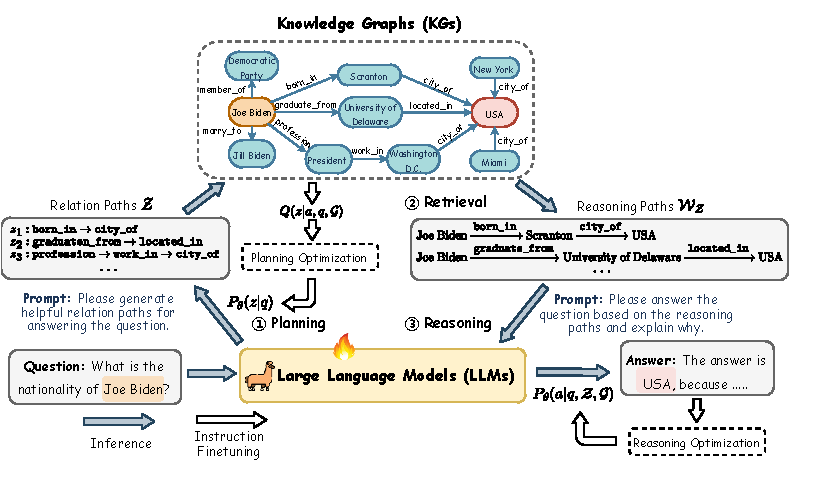
\includegraphics[width=.85\columnwidth]{images/RoG.pdf}
    \end{center}
    \vspace{-3mm}
    \caption{The overall framework of reasoning on graphs (\ourmethod). \RE{1) given a question, we first prompt LLMs to generate several relation paths that are grounded by KGs as plans. 2) Then, we retrieve reasoning paths from KGs using the plans. 3) Finally, we conduct faithful reasoning based on the retrieved reasoning paths and generate answers with interpretable explanations. The orange and red rectangles denote the entities mentioned in the question and answer, respectively.}}
    \label{fig:framework}
    \vspace{-5mm}
\end{figure}

\section{Approach}
% In this section, we introduce our method: reasoning on graphs (\ourmethod). We present a novel \textit{planning-retrieval-reasoning} framework that synergizes LLMs and KGs to conduct faithful and interpretable reasoning for KGQA. The overall framework of \ourmethod is illustrated in \Cref{fig:framework}.


\RE{In this section, we introduce our method: reasoning on graphs (\ourmethod), which contains two components: 1) a \textit{planning} module that generates relation paths grounded by KGs as faithful plans; 2) a \textit{retrieval-reasoning} module that first retrieves valid reasoning paths from KGs according to the plans, then conducts faithful reasoning based on retrieved reasoning paths and generates answers with interpretable explanations. The overall framework of \ourmethod is illustrated in \Cref{fig:framework}.}


\subsection{Reasoning on Graphs: Planning-Retrieval-Reasoning}

Recently, many techniques have been explored to improve the reasoning ability of LLMs by planning, which first prompts LLMs to generate a reasoning plan and then conduct reasoning based on it \citep{wang2023plan}. However, LLMs are known for having hallucination issues, which are prone to generating incorrect plans and leading to wrong answers \citep{ji2023survey}.
%
To address this issue, we present a novel \textit{planning-retrieval-reasoning} framework, which makes the reasoning plans grounded by KGs and then retrieves faithful reasoning paths for LLM reasoning. 

Relation paths, which capture semantic relations between entities, have been utilized in many reasoning tasks on KGs \citep{wang2021relational,xusubgraph}. Moreover, compared to the dynamically updated entities, the relations in KGs are more stable \citep{wang2023survey}. By using relation paths, we can always retrieve the latest knowledge from KGs for reasoning. Therefore, relation paths can serve as faithful plans for reasoning the answer to KGQA task.
\begin{example}
    Given a question ``Who is the child of Alice'', we can generate a relation path as the plan: $z=\texttt{marry\_to} \to \texttt{father\_of}$. This relation path expresses the plan: 1) find the person that ``Alice'' is married to; 2) find the child of that person.
    We can execute the plan (relation path) by retrieving a reasoning path from KGs as: $w_z=\text{Alice}\xrightarrow{\texttt{marry\_to}}\text{Bob}\xrightarrow{\texttt{father\_of}}\text{Charlie}$. Finally, we can answer the question based on the reasoning path, which is ``Charlie''.
\end{example}

By treating relation paths as plans, we can make sure the plans are grounded by KGs, which enables LLMs to conduct faithful and interpretable reasoning on graphs. In a nutshell, we formulate our \ourmethod as an optimization problem that aims to maximize the probability of reasoning the answer from a knowledge graph $\gG$ w.r.t the question $q$ by generating relation paths $z$ as the plan:
% Thus, the objective function of our \ourmethod can be formulated as
\begin{equation}
    \setlength\abovedisplayskip{1pt}%shrink space
    \setlength\belowdisplayskip{1pt}
    \label{eq:plan}
    P_\theta(a|q,\gG) = \sum_{z\in\gZ}P_\theta(a|q,z,\gG)P_\theta(z|q),
\end{equation}
where $\theta$ denotes the parameters of LLMs, $z$ denotes the relation paths (plans) generated by LLMs, and $\gZ$ denotes the set of possible relation paths. The latter term $P_\theta(z|q)$ is the probability of generating a faithful relation path $z$ grounded by KG, given the question $q$, which is realized by the \textit{planning} module. The former term $P_\theta(a|q,z,\gG)$ is the probability of reasoning an answer $a$ given the question $q$, relation path $z$, and KG $\gG$, which is computed by the \textit{retrieval-reasoning} module.

\subsection{Optimization Framework}
Despite the advantage of generating relation paths as plans, the LLMs have zero knowledge of the relations contained in KGs. Therefore, LLMs cannot directly generate relation paths grounded by KGs as faithful plans. Moreover, LLMs might not understand the reasoning paths correctly and conduct reasoning based on them. To address these issues, we design two instruction tuning tasks: 1) \textit{planning optimization}, which distills the knowledge from KGs into LLMs to generate faithful relation paths as plans; 2) \textit{retrieval-reasoning optimization}, which enables LLMs to reason based on the retrieved reasoning paths.

The objective function in \eqref{eq:plan} can be optimized by maximizing the evidence lower bound (ELBO) \citep{jordan1999introduction}, which is formulated as
\begin{equation}
    \log P(a|q,\gG) \geq \E_{z\sim Q(z)}[\log P_\theta(a|q,z,\gG)] - \KL(Q(z)\Vert P_\theta(z|q)),
\end{equation}
where $Q(z)$ denotes the posterior distribution of faithful relation paths grounded by KGs. The latter term minimizes the KL divergence between the posterior and the prior, which encourages LLMs to generate faithful relation paths (planning optimization). The former term maximizes the expectation that retrieval-reasoning module generates correct answers based on the relation paths and KGs (retrieval-reasoning optimization). 

\noindent\textbf{Planning optimization.} In planning optimization, we aim to distill the knowledge from KGs into LLMs to generate faithful relation paths as plans. This can be achieved by minimizing the KL divergence with the posterior distribution of faithful relation paths $Q(z)$, which can be approximated by the valid relation paths in KGs. 

Given a question $q$ and answer $a$, we could find the path instances $w_z(e_q,e_a)=e_q\xrightarrow{r_1}e_1\xrightarrow{r_2}\ldots\xrightarrow{r_l}e_{a}$ connecting $e_q$ and $e_a$ in KGs. The corresponding relation path $z=\{r_1,r_2,\dots,r_l\}$ can be considered valid and serve as a faithful plan for answering the question $q$. The posterior distribution $Q(z)$ can be formally approximated as
\begin{equation}
    \setlength\abovedisplayskip{1pt}%shrink space
    \setlength\belowdisplayskip{1pt}
    \label{eq:posterior}
    Q(z) \simeq Q(z|a, q, \gG)=
    \left\{
    \begin{aligned}
         & \RE{\frac{1}{|\mathcal{Z}|}}, \exists w_z(e_q,e_a) \in \gG, \\
         & 0, else,
    \end{aligned}
    \right.
\end{equation}
where \RE{ we assume a uniform distribution over all valid relation paths $\mathcal{Z}$}, and $\exists w_z(e_q,e_a) \in \gG$ denote the existence of a path instance connecting the question $e_q$ and answer $e_a$ entities in $\gG$.
%
Therefore, the KL divergence can be calculated as
\begin{equation}
    \setlength\abovedisplayskip{1pt}%shrink space
    \setlength\belowdisplayskip{1pt}
    \label{eq:kl}
    \gL_{\text{plan}}=\KL(Q(z)\Vert P_\theta(z|q)) = \KL(Q(z|a, q, \gG)\Vert P_\theta(z|q)) \RE{~\simeq - \frac{1}{|\gZ^*|}\sum_{z\in\gZ^*} \log P_\theta(z|q),}
\end{equation}
\RE{where we use the shortest paths $\gZ^*\subseteq\mathcal{Z}$ between $e_q$ and $e_a$ in KGs as supervision signals \citep{zhang2022subgraph}.} The detailed derivation of can be found in \Cref{app:planning_derivation}.
By optimizing the \eqref{eq:kl}, we maximize the probability of LLMs generating faithful relation paths through distilling the knowledge from KGs.

\noindent\textbf{Retrieval-reasoning optimization.} In retrieval-reasoning optimization, we aim to enable LLMs to conduct reasoning based on the retrieved reasoning paths. 
For the retrieval-reasoning module, we follow the FiD framework \citep{izacard2021leveraging,singh2021end}, which allows reasoning on multiple retrieved reasoning paths\footnote{\RE{The FiD framework assumes each $z\in \mathcal{Z}$ contributes independently, where the probability $P_\theta(a|q,\mathcal{Z},\mathcal{G})$ can be approximated as the product of each $P_\theta(a|q,z,\gG)$.}}, formulated as
\begin{equation}
    \setlength\abovedisplayskip{1pt}%shrink space
    \setlength\belowdisplayskip{1pt}
    P_\theta(a|q,\gZ,\gG) = \prod_{z\in\gZ}P_\theta(a|q,z,\gG).
\end{equation}

By approximating the expectation with \RE{K sampled plans $\gZ^{*}_{K}\subseteq Z^*$}, the objective function of reasoning optimization can be written as
\begin{equation}
    \setlength\abovedisplayskip{1pt}%shrink space
    \setlength\belowdisplayskip{1pt}
    \gL_{\text{reason}}= \E_{z\sim Q(z|a, q, \gG)}[\log P_\theta(a|q,z,\gG)] \RE{ = \sum_{z\in\gZ^*_K} \log P_\theta(a|q,z,\gG)} =  \log P_\theta(a|q,\gZ^*_{K},\gG).
\end{equation}
This maximizes the probability of LLMs generating correct answers based on the retrieved reasoning paths.

The final objective function of \ourmethod is the combination of the planning optimization and retrieval-reasoning optimization, which can be formulated as
\begin{equation}
    \setlength\abovedisplayskip{1pt}%shrink space
    \setlength\belowdisplayskip{1pt}
    \label{eq:final_obj}
    \gL = \log \underbrace{P_\theta(a|q,\RE{\gZ^*_K},\gG)}_{\text{Retrieval-reasoning}} + \underbrace{\RE{\frac{1}{|\gZ^*|}}\sum_{z\in \RE{Z^*}}\log P_\theta(z|q)}_{\text{Planning}}.
\end{equation}
From \eqref{eq:final_obj}, we can see that we adopt the same LLM for both planning and reasoning, which are jointly trained on two instruction-tuning tasks, i.e., (planning and retrieval-reasoning). We will discuss the implementation details of these two tasks in the following subsections.

\subsection{Planning Module}
The planning module aims to generate faithful relation paths as plans for answering the question. To utilize the instruction-following ability of LLMs \citep{wei2021finetuned}, we design a simple instruction template that prompts LLMs to generate relation paths:

% \LH{Any better way to present the instruction template?}
\begin{minipage}{0.99\columnwidth}
    \centering
    \begin{tcolorbox}
        \small
        Please generate a valid relation path that can be helpful for answering the following question: \texttt{<Question>}
    \end{tcolorbox}
    \vspace{1mm}
\end{minipage}
where \texttt{<Question>} indicates the question $q$. The question together with the instruction template is fed into LLMs to generate the relation paths, which are structurally formatted as a sentence:

\begin{minipage}{0.99\columnwidth}
    \centering
    $z=$ \texttt{<PATH>} $r_1$ \texttt{<SEP>}  $r_2$ \texttt{<SEP>} $\dots$ \texttt{<SEP>} $r_l$ \texttt{</PATH>}
    \vspace{1mm}
\end{minipage}
where \texttt{<PATH>}, \texttt{<SEP>}, \texttt{</PATH>} are special tokens indicating the start, separator, and end of the relation path, respectively\footnote{The relation name $r_*$ could be split into multiple tokens. For example, ``\texttt{born\_in}'' could be split into ``\texttt{born}'' and ``\texttt{\_in}'' by tokenizer. In this way,  we could fully utilize the semantic information in relation names and generalize to different KGs.}. 

Therefore, the optimization of $\gL_{\text{plan}}$ can be achieved as
\begin{equation}
    \setlength\abovedisplayskip{1pt}%shrink space
    \setlength\belowdisplayskip{1pt}
    \argmax_\theta \RE{\frac{1}{|\gZ^*|}}\sum_{z\in \RE{\gZ^*}} \log P_\theta(z|q)= \RE{\frac{1}{|\gZ^*|}} \sum_{z\in \RE{\gZ^*}}\log \prod_{i=1}^{|z|}P_\theta(r_i|r_{<i},q),
\end{equation}
where $P_\theta(z|q)$ denotes the prior distribution of generating faithful relation path $z$, and $P_\theta(r_i|r_{<i},q)$ denotes the probability of each token in $z$ generated by LLMs.

\subsection{Retrieval-Reasoning Module}

\noindent\textbf{Retrieval}. Given a question $q$ and a relation path as plan $z$, the retrieval module aims to retrieve the reasoning paths $w_z$ from KG $\gG$. The retrieval process can be conducted by finding paths in $\gG$ that start from the question entities $e_q$ and follow the relation paths $z$, formulated as
\begin{equation}
    \setlength\abovedisplayskip{1pt}%shrink space
    \setlength\belowdisplayskip{1pt}
    \gW_z=\{w_z(e_q,e_*)|w_z(e_q,e_*)=e_q\xrightarrow{r_1}e_1\xrightarrow{r_2}\ldots\xrightarrow{r_l}e_{a*}, w_z(e_q,e_*)\in\gG\}.
\end{equation}
We adopt a constrained breadth-first search to retrieve the reasoning paths $w_z$ from KGs. In experiments, all retrieved paths are used for reasoning. The detailed retrieval algorithm can be found in \Cref{app:retrieval}.

Despite we can utilize the retrieved reasoning paths and directly get the answers with majority voting. The retrieved reasoning paths could be noisy and irrelevant to the questions, which leads to incorrect answers \citep{he2021improving,zhang2022subgraph}. Therefore, we propose a reasoning module to explore the ability of LLMs to identify the important reasoning paths and answer the questions based on them.
% The probability of retrieving the reasoning path $w_z$ from KGs given the relation path $z$ is formulated as
% \begin{equation}
%     \label{eq:posterior}
%     P(w_z|z,q,\gG)
%     \left\{
%     \begin{aligned}
%          & 1, \exists w_z(e_q,e_*) \in \gG, \\
%          & 0, else.
%     \end{aligned}
%     \right.
% \end{equation}

\noindent\textbf{Reasoning}. The reasoning module takes the question $q$ and a set of reasoning paths $\gW_z$ to generate answers $a$. 
Similarly, we design a reasoning instruction prompt to guide LLMs to conduct reasoning based on the retrieved reasoning paths $\gW_z$. The $\gW_z$ are also formatted as a series of structural sentences.
%
% where \texttt{<Reasoning Paths>} denotes the retrieved reasoning paths $\gW_z$ which are formatted as a series of structural sentences.
%
% \begin{minipage}{0.99\columnwidth}
%     \centering
%     $x_z=e_1 \to r_1 \to e_2 \to \dots \to r_l \to e_l,w_z\in\gW_z$.
%     \vspace{1mm}
% \end{minipage}
The detailed prompt can be found in \Cref{app:prompts}. 

The optimization of $\gL_{\text{reason}}$ can be written as
\begin{equation}
    \setlength\abovedisplayskip{1pt}%shrink space
    \setlength\belowdisplayskip{1pt}
    \argmax_\theta \log P_\theta(a|q,\RE{\gZ^*_K},\gG) =  \log \sum_{z\in\RE{\gZ^*_K}}\sum_{w_z\in\gW_z}\prod_{i=1}^{|a|}P_\theta(t_i|t_{<i},q,w_z),
\end{equation}
where $P_\theta(a|q,\gZ_K,\gG)$ denotes probability of reasoning the correct answer $a$ based on $K$ relation paths $\gZ_K$, and $t_*$ denote the tokens of answers $a$.

% \subsection{Optimization}

% The \eqref{eq:plan} can be optimized by maximizing the evidence lower bound (ELBO) \citep{jordan1999introduction}, which can be formulated as
% \begin{equation}
%     \log P(a|q,\gG) \geq \E_{z\sim Q(z)}[\log P_\theta(a|q,z,\gG)] - \KL(Q(z)\Vert P_\theta(z|q)),
% \end{equation}
% where $Q(z)$ denotes the posterior distribution of faithful reasoning plans grounded by KGs. The first term maximizes the expectation that retrieval-then-reasoning module generates correct answers based on the plans. The second term minimizes the KL divergence between the posterior and the prior, which distills the knowledge from KGs and encourages LLM to generate faithful reasoning plans.

% The posterior distribution of faithful plans $Q(z)$ can be approximated by valid relation paths on KGs. Given a question $q$ and answer $a$, we found the shortest paths $w_z(e_q,e_a)=e_q\xrightarrow{r_1}e_1\xrightarrow{r_2}\ldots\xrightarrow{r_l}e_{a}$ connecting $e_q$ and $e_a$ in KGs. Therefore, the valid relation path $z=\{r_1,r_2,\dots,r_l\}$ can be served as a faithful plan for answering the question $q$ and the posterior distribution $Q(z)$ can be formally approximated as
% \begin{equation}
%     \label{eq:posterior}
%     Q(z) \simeq Q(z|a, q, \gG)=
%     \left\{
%     \begin{aligned}
%          & 1, \exists w_z(e_q,e_a) \in \gG, \\
%          & 0, else.
%     \end{aligned}
%     \right.
% \end{equation}

% Therefore, the KL divergence can be calculated as
% \begin{equation}
%     \begin{aligned}
%         \KL(Q(z)\Vert P_\theta(z|q)) &= \KL(Q(z|a, q, \gG)\Vert P_\theta(z|q)) \\
%         &= \E_{z\sim Q(z|a, q, \gG)}Q(z|a, q, \gG)[\log Q(z|a, q, \gG)-\log P_\theta(z|q)] \\
%         &=-\E_{z\sim Q(z|a, q, \gG)}Q(z|a, q, \gG)\log P_\theta(z|q) + \text{CONST}\\
%         &\geq - \sum_{z\in Q(z|a, q, \gG)}\log P_\theta(z|q).
%     \end{aligned}
% \end{equation}

% For the retrieval-then-reasoning module, we follow the FiD model \citep{izacard2021leveraging}, which allows reasoning on multiple retrieved reasoning paths, which is formulated as
% \begin{equation}
%     P_\theta(a|q,\gZ,\gG) = \prod_{z\in\gZ}P_\theta(a|q,z,\gG).
% \end{equation}

% By approximating the expectation with K sampled plans $\gZ_{K}$, the final 
% objective function can be written as
% \begin{equation}
%     \label{eq:final_obj}
%     \gL = \log P_\theta(a|\gZ_K,q,\gG) + \sum_{z\in Q(z|a, q, \gG)}\log P_\theta(z|q).
% \end{equation}
% From \eqref{eq:final_obj}, we can see that we adopt the same LLMs for both planning and reasoning, which are jointly trained on two instruction-tuning tasks. In this way, we can better distill knowledge from KGs to improve the reasoning ability of LLMs.
